\documentclass[a4paper,12pt]{article}
  \usepackage{graphicx}
  \usepackage{indentfirst}
  \title{Fully Convolutional Networks for Semantic Segmentation}
  \author{Jonathan Long, Evan Shelhamer \emph{et al.}}
  \date{2015}

\begin{document}
  \maketitle

\section{Contributions}

We show that a fully convolutional network (FCN) trained end-to-end, pixels-to-pixels on semantic segmentation exceeds the state-of-the-art without further machinery.

\section{Fully convolutional networks}

A network with only layers of convolution or pooling computes a nonlinear \emph{filter}, which we call a \emph{deep filter} or \emph{fully convolutional network}. An FCN naturally operates on an input of any size, and produces an output of corresponding (possibly resampled) spatial dimensions.

\subsection{Adapting classifiers for dense prediction}

Fully connected layers of typical recognition nets can also be viewed as convolutions with kernels that cover their entire input regions. Doing so casts them into fully convolutional networks that take input of any size and output classification maps.

\subsection{Upsampling is backwards strided convolution}

Upsampling with factor $f$ is convolution with a \emph{fractional} input stride of $1/f$. So long as $f$ is integral, a natural way to upsample is therefore \emph{backwards convolution} (sometimes called \emph{deconvolution}) with an output stride of $f$.

In our experiments, we find that in-network upsampling is fast and effective for learning dense prediction.

\subsection{Patchwise training is loss sampling}

Patchwise training do not yield faster or better convergence for dense prediction. Whole image training is effective and efficient.

\subsection{Segmentation Architecture}

For this investigation, we train and validate on the PASCAL VOC 2011 segmentation challenge. We train with a per-pixel multinomial logistic loss and validate with the standard metric of mean pixel intersection over union, with the mean taken over all classes, including background.

\begin{figure}[ht]
	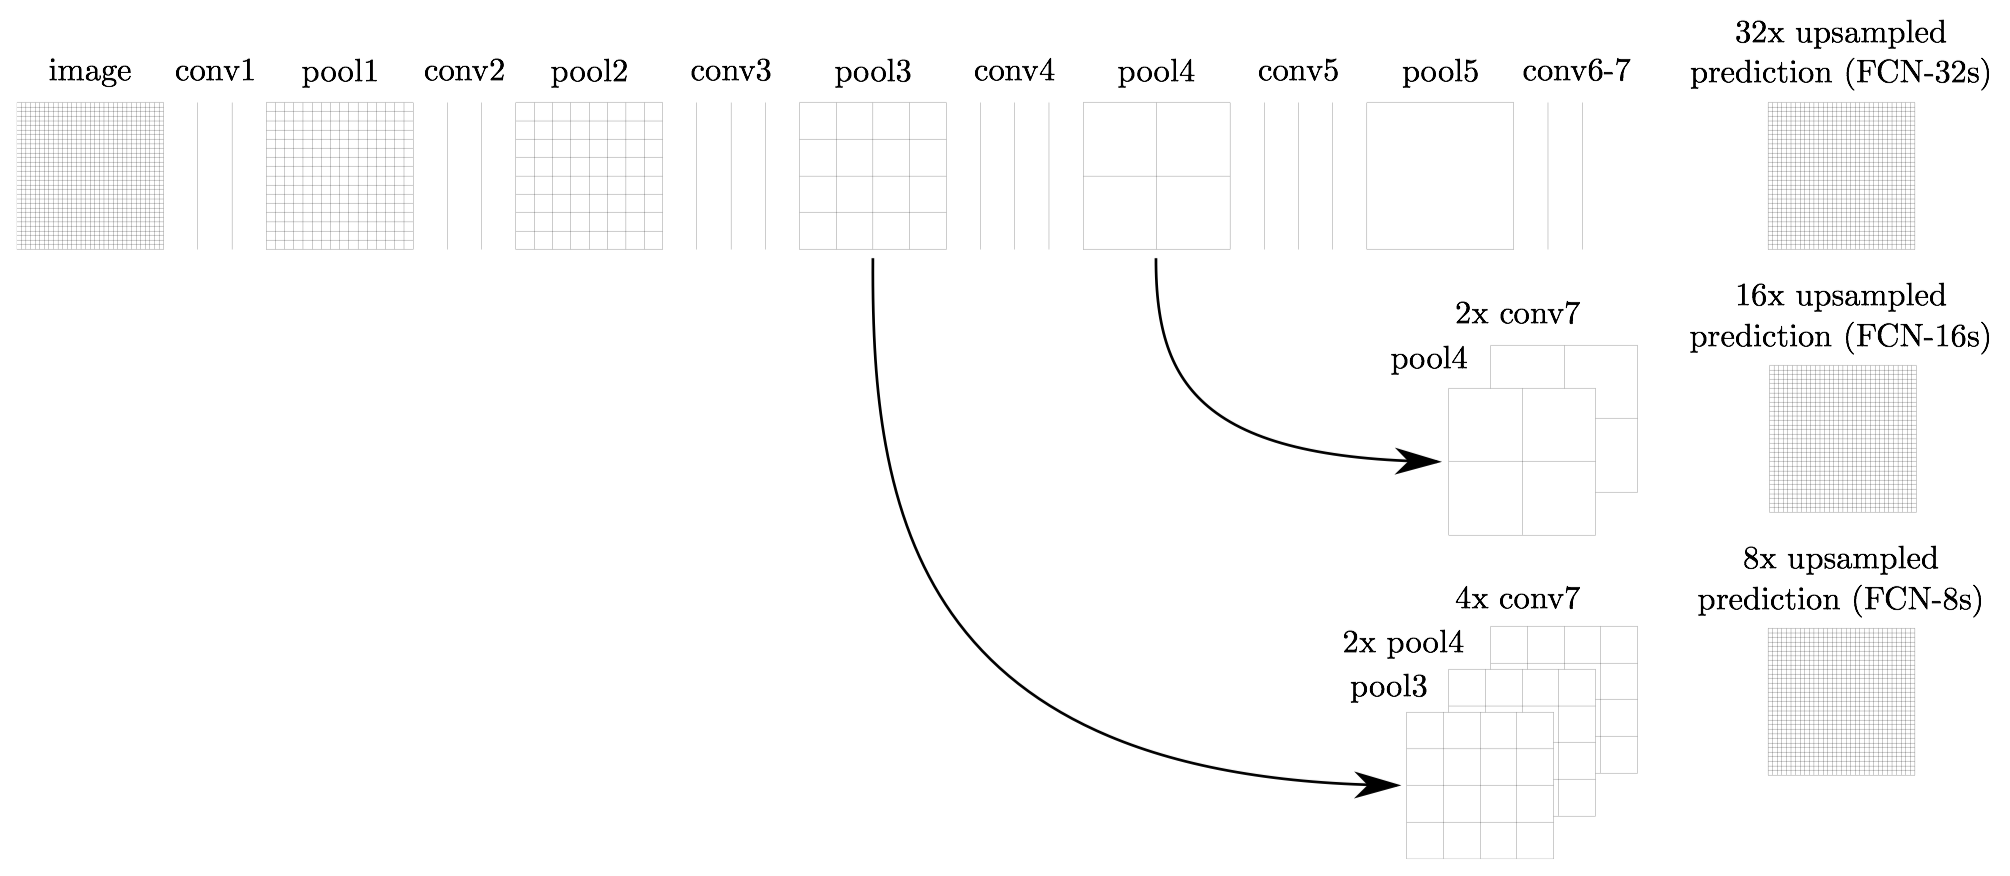
\includegraphics[width=\columnwidth]{fcn.png}
	\caption{Our DAG nets learn to combine coarse, high layer information with fine, low layer information.}
\end{figure}

\subsection{From classifier to dense FCN}

We discard the final classifier layer of each net, and convert all fully connected layers to convolutions. We append a $1 \times 1$ convolution with channel dimension $21$ to predict scores for each of the PASCAL classes (including background) at each of the coarse output locations, followed by a deconvolution layer to bilinearly upsample the coarse outputs to pixel-dense outputs.

Fine-tuning from classification to segmentation gave reasonable predictions for each net.

\subsection{Combining what and where}

While fully convolutionalized classifiers can be fine-tuned to segmentation, and even score highly on the standard metric, their output is dissatisfyingly coarse. We address this by adding skips that combine the final prediction layer with lower layers with finer strides. Combining fine layers and coarse layers lets the model make local predictions that respect global structure.

\section{Conclusion}

Fully convolutional networks are a rich class of models, of which modern classification convnets are a special case. Recognizing this, extending these classification nets to segmentation, and improving the architecture with multi-resolution layer combinations dramatically improves the state-of-the-art, while simultaneously simplifying and speeding up learning and inference.

\end{document}
